A detector can always be tuned to look right on the cases it was tuned on, so the changes were tested on a sample they
were not tuned on, in two ways, and compared with the detector of final v3 (that of \banzai{}~1.1.0). The sample was
re-reduced from raw with the new code into a separate folder (the products of this report are unchanged): all 30 visits
of NGC\,4151 (60 frames), 23 visits of Fairall~9 (46 frames; all visits with a quality flag plus a random selection of
the others) and the 12 BD$+28^\circ4211$ frames with flagged cores. The new code includes the sky-line change of
Section~\ref{sec:cr_sky}, so the COJ frames with the noisy sky change for that reason too.

\subsection{Same-visit test}
\label{sec:cr_pairs}
RM visits have two exposures taken minutes apart. A real cosmic ray is in one of them only; a star core, a line or a
detector defect is in both. For each exposure the other one is shifted along the slit to the same trace position
(difference of the fitted profile centres) and scaled column by column to the same brightness (median ratio over the
trace core, smoothed over 31 columns), and each pixel gets the significance of its excess,
$z=(a-sb)/\sqrt{\sigma_a^2+s^2\sigma_b^2+(0.05\,sb)^2}$, where the 5 per cent allows for small changes of seeing and
position between the exposures. Every connected group of flagged pixels is then classified by its pixel of largest
excess: \textit{real} if $z>6$ and the excess is more than 20 per cent of the signal under it, \textit{false positive}
if all its pixels have $z<3$, \textit{detector} if it is equally high in both exposures at the same detector pixel
(a hot pixel, rightly masked), and \textit{ambiguous} otherwise; groups next to a flag of the other exposure are left
out. Unflagged groups of up to 15 pixels with $z>10$ and an excess over 30 per cent on the object count as
\textit{missed}. Figure~\ref{fig:cr_gallery} shows examples of each class. The test has limits: it cannot judge pixels
on the peak of a very bright line, where a few per cent of change between the exposures is many $\sigma$ (the clipped
H$\alpha$ of Fig.~\ref{fig:cr_halpha} comes out ``ambiguous'', and its flux, not its pixels, shows it was clipped), and
the scaling fails when the seeing changes strongly within a visit (2024 November 30, 11\,arcsec seeing, accounts for
most of the ``missed'' groups of OGG with both detectors).

\begin{figure}[!htbp]
\centering
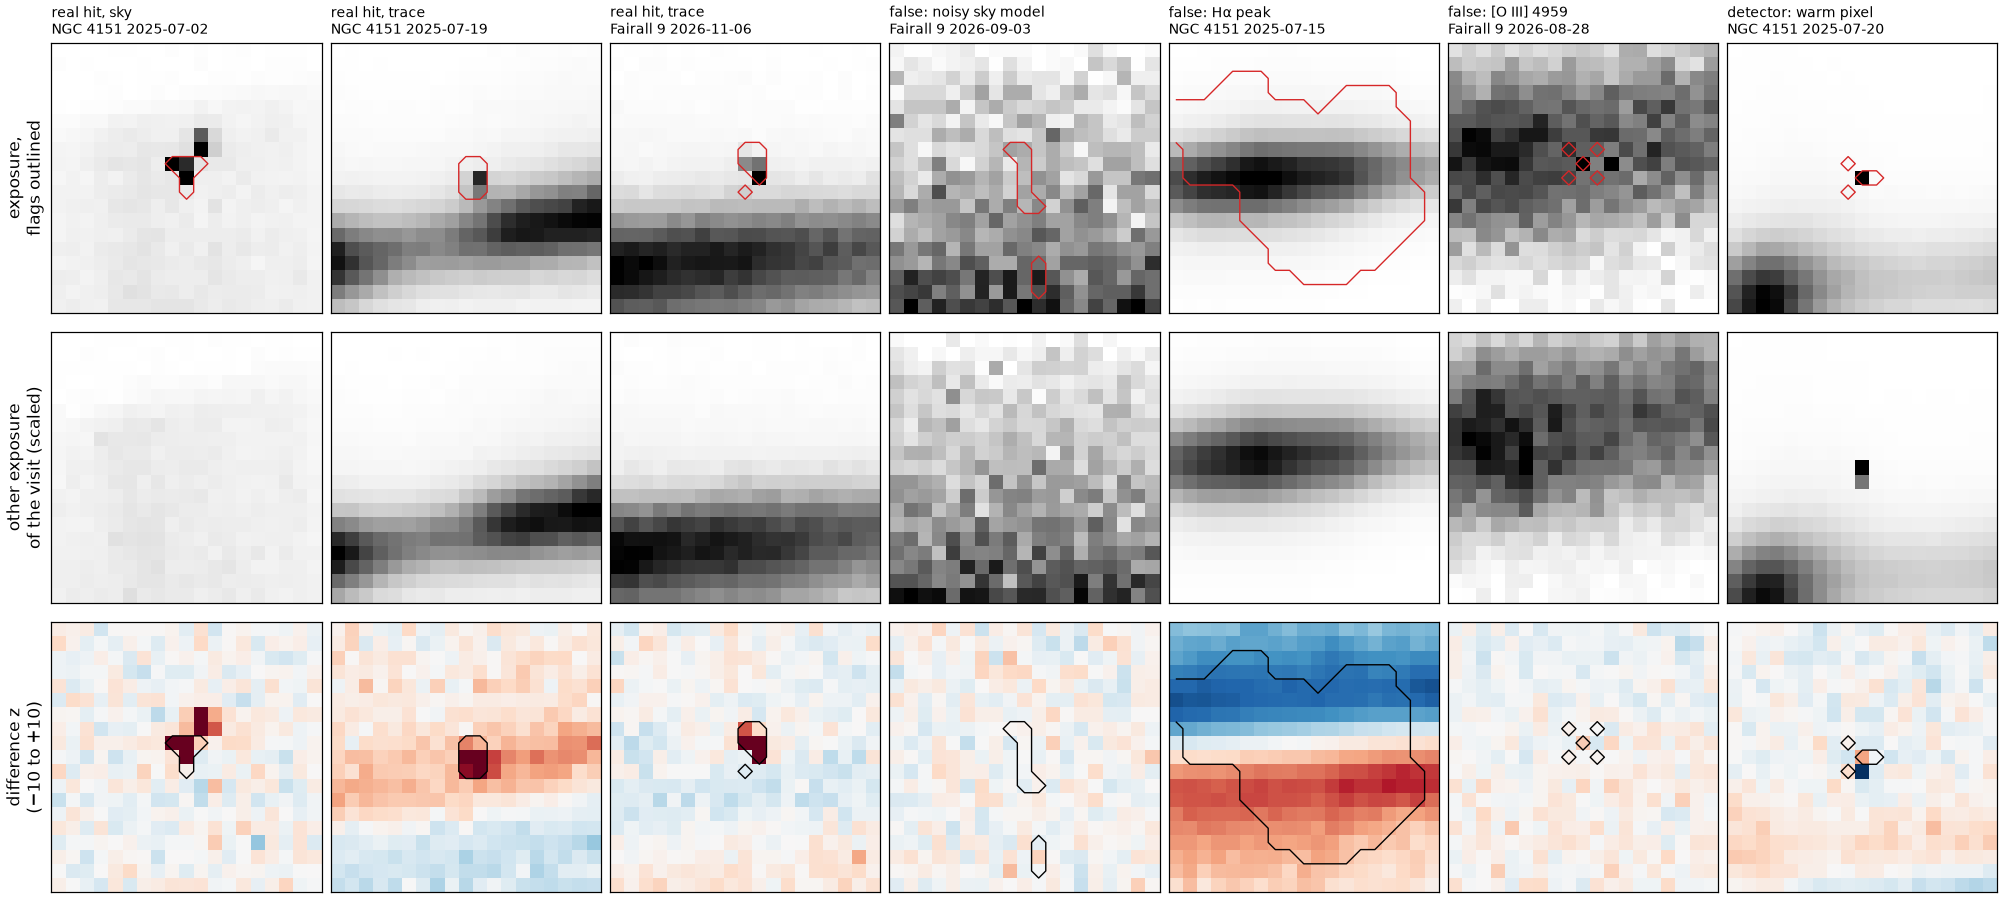
\includegraphics[width=\textwidth]{figures/fig_cr_gallery.png}
\caption{Flagged groups of final v3 classified by the same-visit test. Top: the exposure, flags outlined in red.
Middle: the other exposure of the visit, shifted and scaled onto the first. Bottom: the significance $z$ of the
difference ($-10$ blue to $+10$ red), flags outlined in black. Columns: real hits on the sky and on the trace (a compact
excess absent from the other exposure); false positives from the noisy sky model, on the H$\alpha$ peak (no localised
excess, only the dipole of a sub-pixel shift between the exposures) and on [O\,{\sc iii}]\,4959; and the warm pixel of
the OGG camera, present in both exposures.}
\label{fig:cr_gallery}
\end{figure}

\begin{table}[!htbp]
\centering
\caption{Same-visit test: flagged groups per frame (mean; median in brackets) by class and region, for the detector of
final v3 (\banzai{}~1.1.0) and the new one, on the same frames. ``Object'' is within two FWHM of the trace.}
\label{tab:cr_pairs}
\small
\begin{tabular}{@{}lrrrr@{}}
\toprule
 & \multicolumn{2}{c}{NGC\,4151, OGG (60 frames)} & \multicolumn{2}{c}{Fairall~9, COJ (46 frames)} \\
 & final v3 & new & final v3 & new \\
 & \multicolumn{4}{c}{(groups per frame)} \\
\midrule
real, object & 1.17 (1) & 1.42 (1) & 2.91 (3) & 3.07 (3) \\
false positive, object & 2.72 (1) & 6.30 (5) & 31.2 (6) & 14.8 (10) \\
ambiguous, object & 0.70 (0) & 1.60 (1) & 2.22 (0) & 2.22 (1) \\
missed, object & 11.8 (0) & 11.5 (0) & 1.70 (0) & 1.65 (0) \\
real, sky & 2.35 (2) & 2.35 (2) & 2.54 (2) & 2.65 (2) \\
false positive, sky & 8.87 (9) & 9.53 (9) & 13.2 (9) & 8.46 (8) \\
\bottomrule
\end{tabular}
\end{table}

Table~\ref{tab:cr_pairs} gives the result, and it is mixed:
\begin{itemize}
\item \textit{Real hits} are found as before, slightly more on the object (OGG 70 to 85, COJ 134 to 141 in all), and no
more are missed.
\item \textit{False positives on the object increase in normal frames}: the median per frame goes from 1 to 5 (OGG) and
from 6 to 10 (COJ). The COJ total halves (1435 to 680) only because the frames with the noisy sky model, which had
$\approx240$ each, are fixed. The new false positives are small (median 4 pixels), mostly within one FWHM of the trace
(OGG: 21 groups before, 151 after) and on the continuum, not on lines. Their cause is the other side of the change:
with the object subtracted, the fine-structure test of LA Cosmic is computed on the residual, which is small, and no
longer protects the core of a bright object, so the small pixel-scale structure left in the core of a spectrum with
S/N of a few hundred passes it.
\item \textit{False positives on the sky} are unchanged (OGG) or fewer (COJ, the noisy sky model). They are small groups
of a few faint pixels, cost a few pixels of the sky fit and do not affect the extraction.
\end{itemize}

\subsection{Effect on the extracted fluxes}
\label{sec:cr_flux}
What matters is whether the extra flags change the spectra. Table~\ref{tab:cr_flux} gives the agreement between the two
exposures of each visit, which the flags of either detector can only degrade. The new detector leaves it unchanged
within the noise for [O\,{\sc iii}] in the blue order, for H$\alpha$ and for the continuum, and lowers the bin-to-bin
scatter of the spectra slightly. The worst pairs are the same with both detectors and are grey (clouds, slit losses:
the same ratio in every quantity), except that the new detector removes the clipped H$\alpha$ pair (ratio 0.378). It
creates no new outlier.

The exception is [O\,{\sc iii}]\,5007 of NGC\,4151 in the \textit{red} order, where the line lies only 24\,\AA{} from
the blue end of the order and the dichroic cuts the light steeply: there both detectors clip the line in some frames,
the old one in 2 of 60 (17--22 pixels, flux 4--6 per cent low) and the new one in 6 (5--22 pixels, 4--5 per cent
low); everywhere else the two agree to 0.09 per cent. The bins lose less than half of their profile weight, so the
guard does not catch them. Lines within $\approx30$\,\AA{} of an order end should be measured in the other order, as
[O\,{\sc iii}] normally is in the blue.

\begin{table}[!htbp]
\centering
\caption{Agreement between the two exposures of a visit: robust scatter (per cent) of the ratio of their fluxes, and
the median bin-to-bin scatter of the spectra over their errors (\texttt{L1QXJ}).}
\label{tab:cr_flux}
\small
\begin{tabular}{@{}lrrrr@{}}
\toprule
 & \multicolumn{2}{c}{NGC\,4151 (30 visits)} & \multicolumn{2}{c}{Fairall~9 (23 visits)} \\
 & final v3 & new & final v3 & new \\
\midrule
\multicolumn{5}{@{}l}{\textit{Flux ratio of the two exposures, robust scatter (\%)}}\\
{[O\,{\sc iii}]\,5007}, blue order & 1.99 & 1.93 & 6.7 & 6.8 \\
{[O\,{\sc iii}]\,5007}, red order & 1.71 & 2.49 & 6.7 & 6.6 \\
H$\alpha$+[N\,{\sc ii}] & 2.53 & 2.29 & -- & -- \\
continuum 4200--4500\,\AA{} & 1.49 & 1.56 & 3.3 & 3.6 \\
continuum 7400--7550\,\AA{} & 1.48 & 1.55 & 3.0 & 2.8 \\
\multicolumn{5}{@{}l}{\textit{Bin-to-bin scatter over errors (no unit; 1 = correct)}}\\
scatter / errors (median) & 1.33 & 1.31 & 1.13 & 1.10 \\
\bottomrule
\end{tabular}
\end{table}

\subsection{Injection test}
\label{sec:cr_inject}
The same-visit test cannot see hits on bright line peaks, and it measures false positives better than completeness.
We therefore added 720 synthetic cosmic rays to copies of six raw frames (NGC\,4151 2025-07-15 and 2025-07-20,
BD$+28^\circ4211$ 2025-07-28 and 2025-08-19, Fairall~9 2026-09-06 and 2026-10-08; two random sets each), 20 per frame
in each of three places: the \textit{sky} (more than 3\,FWHM from the trace), the \textit{trace} (within 1\,FWHM, away
from the brightest pixels) and the \textit{peak} (the brightest 3 per cent of the trace core: the line peaks of the AGN
and the core of the star). The hits had peak charges from 50 to 20\,000\,e$^-$ (log-uniform) and the shapes of real
ones (one pixel, two pixels or a short track). Each copy, and the frame without hits, was reduced with both detectors;
a hit counts as detected if any of its pixels is flagged. Figure~\ref{fig:cr_validation} and
Table~\ref{tab:cr_inject} give the result:
\begin{itemize}
\item On the \textit{sky} both detectors find the same 90 per cent of the hits above 10$\sigma$ (the misses are the same
21 hits for both, 14 of them in the 2-pixel band at the order edges that is excluded from the search).
\item On the \textit{trace}, above 10$\sigma$, the old detector finds 89 per cent and the new one 100 per cent.
\item On the \textit{peaks} the old detector finds only 66 per cent of the hits above 10$\sigma$, and in the brightest
frames almost none: of the hits above 20$\sigma$, 0 of 8 on the core of BD$+28^\circ4211$ (2025 July 28) and 2 of 10 on
the H$\alpha$ peak of NGC\,4151 (2025 July 15). The new detector finds 97 per cent (83--100 per cent in every frame).
\item The masks cover the hits equally (95--97 per cent of the pixels of a detected hit), and when hits are added the
old detector also flags 49 pixels per frame that are not on a hit, the new one 13: with the low growth threshold
(step 6), a detection near a bright region spreads into it.
\end{itemize}
The reason is the same as for the false positives above, seen from the other side: the fine-structure test that
protected the object also hid the cosmic rays on it, because a hit on a bright core or line is a small sharp excess on
a large sharp signal. With the object subtracted, the hit stands out. A single hit on the [O\,{\sc iii}] peak of NGC\,4151
missed by the new detector in a first test (Section~\ref{sec:cr_model}) was one of the 3 per cent.

\begin{table}[!htbp]
\centering
\caption{Injection test: fraction of the injected cosmic rays detected (720 hits in six frames, each reduced with both
detectors).}
\label{tab:cr_inject}
\small
\begin{tabular}{@{}lrrrr@{}}
\toprule
 & \multicolumn{2}{c}{hits above 10$\sigma$} & \multicolumn{2}{c}{hits of 5--10$\sigma$} \\
place & final v3 & new & final v3 & new \\
 & \multicolumn{4}{c}{(fraction of the hits detected)} \\
\midrule
sky (240 hits) & 0.90 & 0.90 & 0.92 & 0.92 \\
trace (240) & 0.89 & 1.00 & 0.47 & 0.60 \\
line peak or star core (234) & 0.66 & 0.97 & 0.19 & 0.67 \\
\midrule
flags not on a hit (pixels per frame) & 49 & 13 & & \\
\bottomrule
\end{tabular}
\end{table}

\begin{figure}[!htbp]
\centering
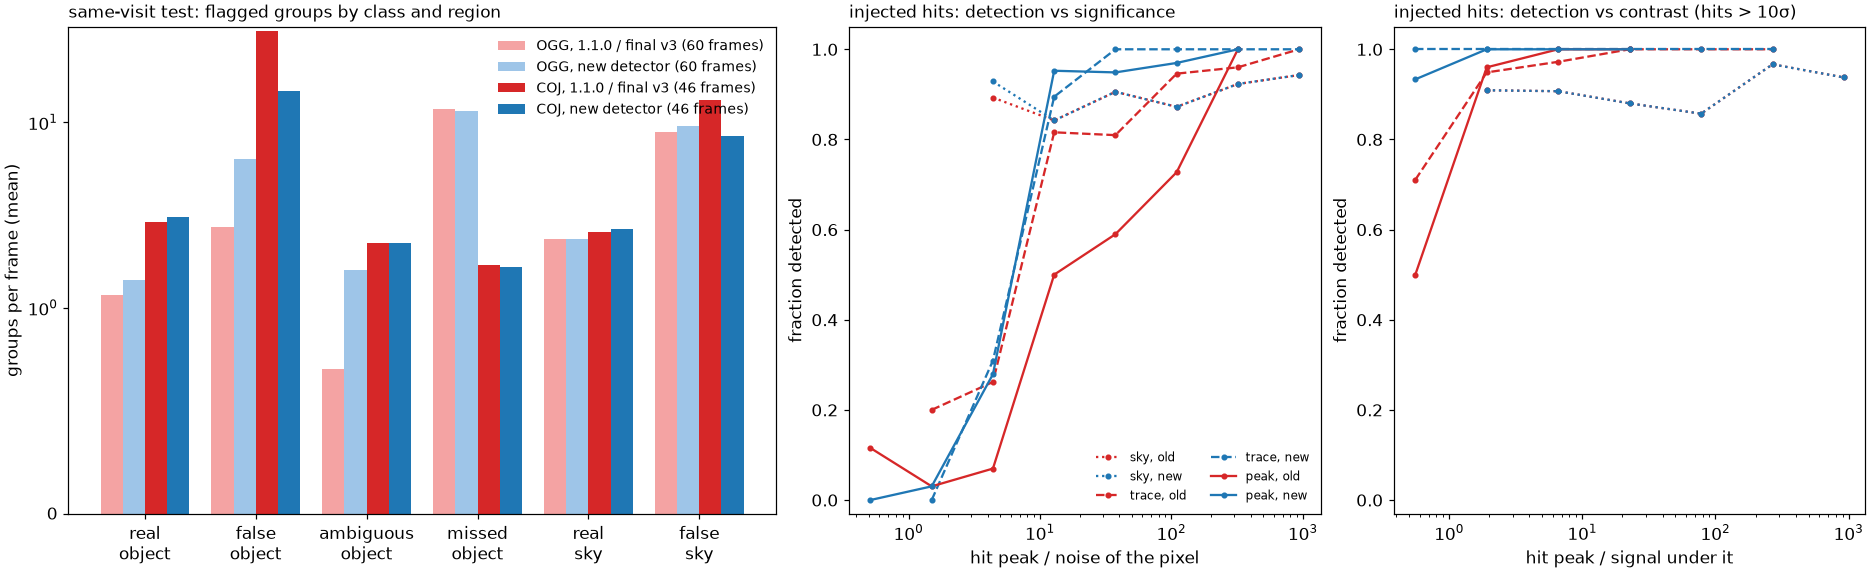
\includegraphics[width=\textwidth]{figures/fig_cr_validation.png}
\caption{Verification of the new detector against that of final v3 (\banzai{}~1.1.0). Left: same-visit test, flagged
groups per frame by class and region (Table~\ref{tab:cr_pairs}; the many ``missed'' groups of OGG are one visit with
11\,arcsec seeing, for both detectors). Middle: fraction of injected hits detected against their significance, on the
sky (dotted), the trace (dashed) and the line peaks or star core (solid), old (red) and new (blue). Right: the same
against the ratio of the hit to the signal under it, for hits above 10$\sigma$.}
\label{fig:cr_validation}
\end{figure}

\subsection{Conclusion}
\label{sec:cr_conclusion}
On the object, the new detector finds more of the real cosmic rays (on bright cores and line peaks 97 instead of 66 per
cent), stops flagging the cores of bright stars (46 to 0.1 per cent) and most of the clipped H$\alpha$ (179 to 15 pixels;
flux error 2.64 to 1.02), and removes the false detections caused by a noisy sky. In exchange it adds a few small false
detections per frame on the trace of bright objects (median 1 to 5 at OGG), which leave the extracted fluxes unchanged
within the noise, except for lines within $\approx30$\,\AA{} of an order end, where both detectors clip (2 and 6 frames of
60). On balance it is better on every measure that affects the spectra, but it is not perfect, and the results depend
on the parameters of LA Cosmic, which were left as in \banzai{}. A single frame cannot reliably separate a cosmic ray
from the peak of a bright line; the two or more exposures of every RM visit can, and comparing them is the robust
solution we recommend (Chapter~\ref{sec:recommendations}). We have not re-reduced the products with the new detector:
that, and whether to adopt it before a comparison of exposures exists, is a decision for the team.

